% !TeX spellcheck = en_GB

\section{Algorithms}\label{algorithms}
\noindent Analogue to the script: \\
grammar $G=(V,\ \Sigma,\ S,\ P)$.\\
$V$ is a finite set of variables. \\
$\Sigma$ is an alphabet. \\
$S$ is the starting symbol and $S \in V$. \\
$P$ is a finite set of rules: $P \subseteq V \times (V \cup \Sigma)^{*}$.\\ 
$G$ is in CNF and therefore it holds, more specifically:  $P\ \subseteq\ V \times\ (V^{2} \cup \Sigma)$. Think about if it is ok. \\
$Vs$ are Variables like "A, B, ...".\\
$(V \cup\ \Sigma)^{*}$ are terminals like "a, b, ..." and compound variables like "AB, BS, AC, ...". \\
$i,j \in \mathbb{N};\ [i,\ j] := \{i,\ i+1,..., j-1,\ j\} \subseteq \mathbb{N}_{\geq 0}$. $word \in \Sigma^* $ \\
$Pyramid :=\{ cell_{i,j}\ |\ i \in \mathbb{N}_{\geq 0},\  j \in [0,\ j_{max}-i],\ i_{max} = j_{max} = |word|-1\}$.\\
$cell_{i,j} = \{Cell_{i,j}\ |\ Cell_{i,j} \subseteq V\}$. If each $cell_{i,j}=\emptyset$ then it is called $EmptyPyramid$.\\
Note that regarding one $cell_{i,j}$: $cell_{i,j} = cellDown$, $cell_{i-1,j} = cellUpperLeft$ and $cell_{i-1,j+1} = cellUpperRight$  \\
Multisets allow duplicate elements. Notation of a multiset is done via the index b, that stands for bag: $multiset_b$\\


\begin{figure}[h]
	\centering
	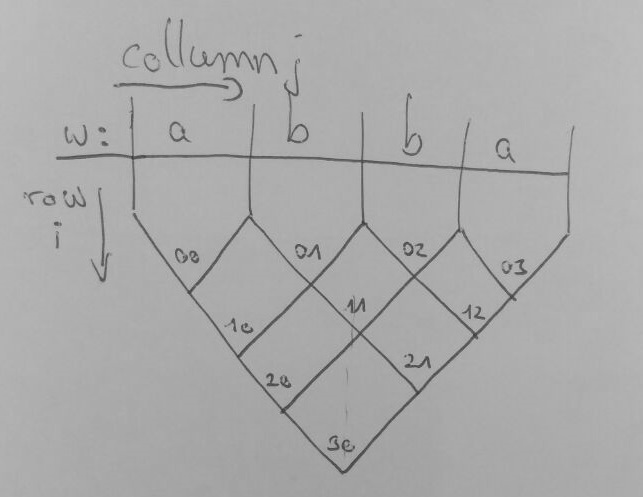
\includegraphics[width=0.7\textwidth]{abb/DataStructurePyramid}
\end{figure}
 \pagebreak 
\noindent
\frame{
	\begin{algorithm}[H] %or another one check
		\caption{distributeRhse}
		\label{distributeRhse}
		\SetAlgoLined
		\KwIn{ $G,\ Rhse \subseteq\ (V^{2} \cup \Sigma),\ i,\ j$}
		\KwOut{$Grammar\ G\ with\ uniform\ randomly\ distributed\ Rhse's.$}
		\ForEach {$rhse \in Rhse$}{
			$choose\ n\ uniform\ randomly\ in\ [i, j]$\;
			$choose\ V_{add} := uniform\ random\ subset\ of\ size\ n\ from\ V$\;
			$G.P = G.P\ \cup\ \{ "v\longrightarrow rhse"\ |\ v \in V_{add} \} $\;	
		}
		\Return $G$;
	\end{algorithm}
}
\\
\\
\frame{
	\begin{algorithm}[H] %or another one check
		\caption{calculateSubsetForCell}
		\label{calculateSubsetForCell}
		\SetAlgoLined
		\KwIn{$Pyramid,\ cell_ {i,j} $}
		\KwOut{$V_{i,j} \subseteq V^2$}
		$V_{i,j} = \emptyset $\;
		\For{$m:=i-1 \to 0$}{
			$V_{i,j} = V_{i,j} \cup \{X\ |\ X\longrightarrow YZ,\ Y \in V_{m,j},\ Z \in V_{i-m-1,m+j+1} \}$\;
		}
		
		\Return $V_{i,j}$;
		\end{algorithm}
}
\noindent
\\
\\
\frame{
	\begin{algorithm}[H] %or another one check
		\caption{checkForceCombinationForCell}
		\label{checkRightCellCombination}
		\SetAlgoLined
		\KwIn{$ cell_{i,j}\subseteq V^2 \, cell_{i-1,j}\subseteq V^2,\ cell_{i-1,j+1} \subseteq V^2,\ G.P $ }
		\KwOut{$varsForcing\subseteq V$}
		$varsForcing = \emptyset$\;
		$varComp = \{XY\ |\ X \in cell_{i-1,j}\ \wedge\ Y \in cell_{i-1,j+1} \}$\;
		\ForEach{$v \in cellDown$}{
			$prods = \{p\ |\ v \in G.P.V \}$\;
			$rhses = \{rhse\ |\ rhse \in prods.(V^{2} \cup \Sigma) \} $\;
			\If{$varComp \nsubseteq rhses$}{
				$varsForcing = varsForcing\ \cup\ v$\;
			}			
		}
		\Return $varsForcing$\;
		\footnotetext{Input: $cell_{i,j} = cellDown$, $cell_{i-1,j} = cellUpperLeft$ and $cell_{i-1,j+1} = cellUpperRight$
		}
	\end{algorithm}
}
\\
\\
\frame{
	\begin{algorithm}[H] %or another one check
		\caption{GeneratorGrammarDiceRollMartens}
		\label{GeneratorGrammarDiceRollMartens}
		\SetAlgoLined
		\KwIn{ $word \in \Sigma^{*},\ V,\ \Sigma,\ S,\ P = \emptyset,\ minCount\Sigma,\ maxCount\Sigma,\ $ $ minCountVarComp,\ maxCountVarComp $ }
		\KwOut{$G$}
		
		$G=(V,\Sigma , S, P)$\;
		$G = distributeRhse(G,\ \Sigma,\ minCount\Sigma,\ maxCount\Sigma ) $\;
		$Pyramid = CYK.calculatePyramid(G,\ word)$\;
		\For{$i:=1\ \to\ i_{max}$}{
			\For{$j:=0\ \to\ j_{max}-i$}{
				$sub = calculateSubsetForCell(Pyramid,\ i,\ j)$\;
				\ForEach{$vc \in sub$}{
					\While{$cell_{i_{max},0} = \emptyset$}{
						$distributeRhse(G,\ vc,\ minCountVarComp,\ $ $maxCountVarComp ) $\;
						$Pyramid = CYK.calculatePyramid(G,\ word)$\;	
					}
				}
			}
		}
		\Return $G$\;
		\footnotetext{
		\noindent Line 3: Fills the i=0 row of the pyramid.
			
		\noindent line 5: Instead of going from left to right, choose $j$ uniform randomly with the restrictions that one cell is only visited one time.
		
		\noindent Note: The algorithm tends to finish already within $i = 1$ loop.
		}
	\end{algorithm}
}
\noindent
\frame{
	\begin{algorithm}[H] %or another one check
		\caption{GeneratorGrammarDiceRollMartens2}
		\label{GeneratorGrammarDiceRollMartens2}
		\SetAlgoLined
		\KwIn{ $word \in \Sigma^{*},\ V,\ \Sigma,\ S,\ P = \emptyset,\ minCount\Sigma,\ maxCount\Sigma,\ $ $ minCountVarComp,\ maxCountVarComp $ }
		\KwOut{$G$}
		$G=(V,\Sigma , S, P)$\;
		$G = distributeRhse(G,\ \Sigma,\ minCount\Sigma,\ maxCount\Sigma ) $\;
		$Pyramid = CYK.calculatePyramid(G,\ word)$\;
		$sub = \emptyset$\;
		\For{$i:=1\ \to\ i_{max}$}{
			%$choose\ j\ uniform\ randomly\ in\ [0,\ j_{max}-i]  $\;
			\For{$j:=0\ \to\ j_{max}-i$}{
				$sub = sub \cup \{(A,i)\ |\ A \in calculateSubsetForCell(Pyramid,\ i,\ j) \}$\;
			}
			$sub_b = \{B\ | \ B \in sub,\ sub_b\ models\ i$-$dependent\ priority\ mechanism \} $\;
			\While{$cell_{i_{max},0} = \emptyset \ \wedge\ threshold_i = false $}{
				$choose\ one\ vc\ uniform\ randomly \in sub_b$\;
				$distributeRhse(G,\ vc,\ minCountVarComp,\ $ $maxCountVarComp ) $\;
				$Pyramid = CYK.calculatePyramid(G,\ word)$\;
				$evaluate\ and\ update\ threshold_i$\;	
			}
		}
		\Return $G$\;
		\footnotetext{
			\noindent Line 3: Fills the i=0 row of the pyramid.
			
			\noindent Line 7: $(AB,1), (AB,2), (BC,3) ... \in sub$ $\rightarrow$ multiple occurrences of $AB$ are allowed. This considers "more important" compound variables. 
			
			\noindent Line 11: One vc can be chosen several times.
			
			\noindent Note: Threshold: Linear or log function $f(i)$?
			
			\noindent Note: Priority mechanism: In line $i+1$ the $k = \{(A,l)\ |\ (A,l) \in sub,\ l=i  \}$ are preferred over the\\ $m = \{(A,n)\ |\ (A,n) \in sub,\ n < i  \}$. In what way are they preferred? Using some kind of factor to weight the $i$ of $(A,i)$.
		}
	\end{algorithm}
}
\pagebreak 




\lstset{language=java}
\begin{lstlisting}[frame=htrbl, caption={CYK.calculateSetVAdvanced}, 
label={lst:CYK.calculateSetVAdvanced}]
Algorithm: CYK.calculateSetVAdvanced
Input: grammar, word;
Output: Set<VariableK>[][] cYKMatrix;

Set<VariableK>[][] cYKMatrix = new Set<VariableK>[wordSize][wordSize];
cYKMatrix = calculateCYKMatrix;
return cYKMatrix;
\end{lstlisting}

\pagebreak


\lstset{language=java}
\begin{lstlisting}[frame=htrbl,caption={GeneratorGrammarDiceRollOnly}, 
label={lst:GeneratorGrammarDiceRollOnly}]
Algorithm: GeneratorGrammarDiceRollOnly
Input: settings;
Output: grammar;
Note: A lot of productions are generated, that later on are not needed
for parsing the specific word.

Grammar grammar = new Grammar();
// Part1: Distribute the terminals.
grammar = distributeDiceRollRightHandSideElements(
	grammar, settingsTerminals, minCountTerminals, 
	maxCountTerminals, settingsListVariables);
// Part2: Distribute the compound variables.
Set<Variables> vars = settings.getVariables();
Set<VariablesCompound> setVarComp;
setVarComp = calculate all the possible tupels of ({vars}, {vars});
grammar = distributeDiceRollRightHandSideElements(
	grammar, settingsTerminals, minCountVariableCompound, 
	maxCountVariableCompound, setVarComp);
return grammar
\end{lstlisting}

\pagebreak

\lstset{language=java}
\begin{lstlisting}[frame=htrbl,caption={GeneratorGrammarDiceRollOnlyBias}, 
label={lst:GeneratorGrammarDiceRollOnlyBias}]
Algorithm: GeneratorGrammarDiceRollOnlyBias
Input: settings;
Output: grammar;
Note: A lot of productions are generated, that later on are not needed
for parsing the specific word.

Grammar grammar = new Grammar();
// Distribute the terminals.
grammar = distributeDiceRollRightHandSideElementsBias(
	grammar, settingsTerminals, settingsMinCountTerminals, 
	settingsMCountTerminals, settingsListVars, settingsFavouritism);

// Distribute the compound variables.
Set<VariablesCompound> setVarComp;
setVarComp = calculate all the possible tupels of ({vars}, {vars});
grammar = distributeDiceRollRightHandSideElementsBias(
	grammar, varComp, settingsMinCountVars,
	settingsMaxCountVars, settingsListVars, settingsFavouritism);
return grammar;
\end{lstlisting}

\pagebreak

\lstset{language=java}
\begin{lstlisting}[frame=htrbl,caption={distributeDiceRollRightHandSideElementsBias}, 
label={lst:distributeDiceRollRightHandSideElementsBias}]
Algorithm: distributeDiceRollRightHandSideElementsBias
Input: grammar, setRhse, minCount, maxCount, listVars, favouritismList;
Output: grammar;
Note: Because of dice rolling anyways and lots of grammars being 
generated, no rhse is added if the production already exists.

// Calculate the bloated varSet.
List<Variable> varsBloated;
for(Variables varTemp :  settings.getVariables()){
	tempFavour = randomly pick favouritism[i];
	varsBloated.add({tempFavour times varTemp});
	favouritism.remove(tempFavour);
}
// Because of dice rolling anyways and lot of grammars being generated, 
// just no rhse is added if the production already exists.
grammar = distributeDiceRollRightHandSideElements( grammar,
	varsBloated, minCount, maxCount, listVars );
return grammar;
\end{lstlisting}

\frame{
	\begin{algorithm}[H] %or another one check
		\caption{distributeDiceRollRightHandSideElementsBias}
		\label{distributeDiceRollRightHandSideElementsBias}
		\SetAlgoLined
		\KwIn{ $G,\ rhse \subseteq\ RHSE,\ 0\leq minCount\leq maxCount\leq\ \mid G.V\mid,\ favouritism = \{x\ |\ x\ \epsilon\ \mathrm{N}\ \wedge\ |favouritism| = |G.V| \}$}
		\KwOut{$G$}
		
		$favour = \{(v,\ f )\ |\ v\ \epsilon\ V \wedge\ f\ \epsilon\ favouritism\  \wedge\ tupel\ are\ created\ via\ dice\ roll \}$\;
		$varsBloated_b = \emptyset $\;
		\ForEach{fav in favour}{
			$varsBloated_b = varsBloated_b\ \biguplus\ \{ v^{f} \}$\;
		}
		\Return $distributeDiceRollRhse(
		G ,\ MISTAKEHEREvarsBloated_b,\ minCount,\ maxCount\ )$\;
		
		Still working on. One more Pprameter needed for distributeDiceRollRighthandSideElement. Parameter V that defines the variables the rhse are added to. OR make this algorithm independent.
		\footnotetext{Line 6: Note that $varsBloated_b$ is a multiset, but should actually be a set. Exceptions causing a duplicate production to
		the grammar are not relevant because G.P is a set. }
	\end{algorithm}
}

\pagebreak
\noindent Description of the checks here. \\
\noindent All test of the GrammarValidityChecker class are based on the simple setV matrix. \\

\noindent  isValid = isWordProducible \&\& isExamConstraints \&\& isGrammarRestrictions\\

\noindent  isWordProducible = CYK.algorithmAdvanced()\\

\noindent  isExamConstraints = isRightCellCombinationsForced \&\& isMaxSumOfProductionsCount \&\& isMaxSumOfVarsInPyramidCount \&\& countRightCellCombinationsForced \\

\noindent isGrammarRestrictions = isSizeOfWordCount \&\& isMaxNumberOfVarsPerCellCount \\

\lstset{language=java}
\begin{lstlisting}[frame=htrbl, caption={checksumOfProductions}, 
label={lst:checksumOfProductions}]
Algorithm: checksumOfProductions
Input: grammar, maxSumOfProduction;
Output: isSumOfProductions;

return grammar.getProductionsAsList().size() <= maxSumOfProductions; 
\end{lstlisting}

\pagebreak
\lstset{language=java}
\begin{lstlisting}[frame=htrbl, caption={checkMaxNumberOfVarsPerCell}, 
label={lst:checkMaxNumberOfVarsPerCell}]
Algorithm: checkMaxNumberOfVarsPerCell
Input: setVSimple, maxNumberOfVarsPerCell;
Output: isMaxNumberOfVarsPerCell;
Note: Checking for maxNumberOfVarsPerCell <= zero isn't allowed;

int tempMaxNumberOfVarsPerCell = 0;
int wordLength = tempSetV[0].length;
for ( int i = 0; i < wordLength; i++ ) {
	for ( int j = 0; j < wordLength; j++ ) {
		if ( tempSetV[i][j].size() > numberOfVarsPerCell ) {
			numberOfVarsPerCell = tempSetV[i][j].size();
		}
	}
}
return tempMaxNumberOfVarsPerCell <= maxNumberOfVarsPerCell;
\end{lstlisting}

\pagebreak

\lstset{language=java}
\begin{lstlisting}[frame=htrbl, caption={checkMaxSumOfVarsInPyramid}, 
label={lst:checkMaxSumOfVarsInPyramid}]
Algorithm: checkMaxSumOfVarsInPyramid
Input: setVSimple, maxSumOfVarsInPyramid;
Output: isMaxSumOfVarsInPyramid;

// put all vars of the matrix into one list and use its length.
List<Varaible> allVarsList = new ArrayList<>();
for ( int i = 0; i < setVSimple.length; i++ ) {
	for ( int j = 0; j < setVSimple.length; j++ ) {
		tempVars.addAll( setVSimple[i][j] );
	}
}
return allVarsList.size() <= maxSumOfVarsInPyramid; 
\end{lstlisting}

\pagebreak

\lstset{language=java}
\begin{lstlisting}[frame=htrbl, caption={rightCellCombinationsForced}, 
label={lst:rightCellCombinationsForced}]
Algorithm: rightCellCombinationsForced
Input: setVSimple, minCountForced, grammar;
Output: isForced, countForced, setVSimpleVarsThatForce;
Note: Keep in mind that the setV matrix is a upper right matrix. But the
description of how the algorithm works is done, as if the setV pyramid 
points downwards (reflection on the diagonal + rotation to the left).
Regarding one cell, its upper left cell and its upper right cell 
are looked at. setV[i][j] = down cell. setV[i + 1][j] = upper right cell
setV[i][j - 1] = upper left cell.

int countForced = 0;
Set<Variable>[][] setVMarkedVarsThatForce;
for(Cell cell : setVSimple){
	// Trivial cases that would fulfil the restrictions each time. 
	Ignore the upper two rows of the pyramid; 
	isRightCellCombinationForced = true;
	if(!upperLeftCell.isEmpty() && !upperRightCell.isEmpty()) {
		break;
	}
	setVariableCompound = calculate all the possible tupels of 
		({varLeft}, {varRight});
	for(Variable var : cellToBeVisited) {
		varDownProdList = grammar.getProdList(varDown);
		for(VariableCompound varComp : setVariableCompound) {
			for(Production prod : varDownProdList){
				if(prod.getRhse() == varComp) {
					isForced = false;
				}
			}
		}
		if(isRightCellCombinationForced) {
			rightCellCombinationsForced++;
			// Cell has index i and j.
			setVMarkedVarsThatForce[i][j].add(var)
		}
	}
}
boolean isForced = countForced >= minCountRightCellCombinationsForced;
return isForced, countForced, setVMarkedVarsThatForce;
\end{lstlisting}

\pagebreak

\lstset{language=java}
\begin{lstlisting}[frame=htrbl, caption={Util.removeUselessProductions}, 
label={lst:Util.removeUselessProductions}]
Algorithm: Util.removeUselessProductions
Input: grammar, setVSimple, word
Output: grammar
Note: Very similar to the calculateSetVAdvanced algorithm. Additionally
to storing the k, it is also saved, which production have been used. 
All productions that haven't been need are removed, from the grammar.

Set<Production> allProductions = grammar.getProductions();
Set<Production> onlyUsefulProductions;
onlyUsefulProductions = calculate useful productions with the input of
	grammar, setVSimple and word ;
grammar.remove(allProductions);
return grammar.add(onlyUsefulProductions);
\end{lstlisting}

\pagebreak